\documentclass[journal,12pt,onecolumn]{IEEEtran}
\usepackage{cite}
 \usepackage{caption}
\usepackage{graphicx}
\usepackage{amsmath,amssymb,amsfonts,amsthm}
\usepackage{algorithmic}
\usepackage{graphicx}
\usepackage{textcomp}
\usepackage{xcolor}
\usepackage{txfonts}
\usepackage{listings}
\usepackage{enumitem}
\usepackage{mathtools}
\usepackage{gensymb}
\usepackage{comment}
\usepackage[breaklinks=true]{hyperref}
\usepackage{tkz-euclide} 
\usepackage{listings}
\usepackage{gvv}
%\def\inputGnumericTable{}                                 
\usepackage[latin1]{inputenc} 
\usetikzlibrary{arrows.meta, positioning}
\usepackage{xparse}
\usepackage{color}                                            
\usepackage{array}                                            
\usepackage{longtable}                                       
\usepackage{calc}                                             
\usepackage{multirow}
\usepackage{multicol}
\usepackage{hhline}                                           
\usepackage{ifthen}                                           
\usepackage{lscape}
\usepackage{tabularx}
\usepackage{array}
\usepackage{float}

\usepackage{float}
%\newcommand{\define}{\stackrel{\triangle}{=}}
\theoremstyle{remark}
\usepackage{circuitikz}
\captionsetup{justification=centering}
\usepackage{tikz}

\title{Matrices in Geometry 4.11.13}
\author{EE25BTECH11035 - Kushal B N}
\begin{document}
\vspace{3cm}
\maketitle
{\let\newpage\relax\maketitle}
\textbf{Question: }\\
Find the equation of the plane passing through the points (2,5,-3), (-2,-3,5), and (5,3,-3). Also find the point of intersection of this plane with the line passing through points (3,1,5) and (-1,-3,-1).

\textbf{Given: } \\
The points $\vec{A}\myvec{2\\5\\-3}$, $\vec{B}\myvec{-2\\-3\\5}$ and $\vec{C}\myvec{5\\3\\-3}$ which pass through a plane.\\
The points $\vec{D}\myvec{3\\1\\5}$ and $\vec{E}\myvec{-1\\-3\\-1}$ which pass through a line.

\textbf{Solution: }\\
If $\vec{n}$ is the normal vector to the plane, then by the plane equation we can write\\
\begin{equation}
    \vec{n}^{\top}\vec{A} = c
\end{equation}
\begin{equation}
    \vec{n}^{\top}\vec{B} = c
\end{equation}
\begin{equation}
    \vec{n}^{\top}\vec{C} = c
\end{equation}

which can be writeen as
\begin{equation}
    \myvec{A&B&C}^{\top}\vec{n} = \myvec{1\\1\\1}
\end{equation}
Forming the augmented matrix for this
\begin{equation}
    \augvec{3}{3}{2&5&-3&1\\-2&-3&5&1\\5&3&-3&1}
\end{equation}

\begin{equation}
    \augvec{3}{3}{2&5&-3&1\\-2&-3&5&1\\5&3&-3&1} \xleftrightarrow{R_1 \leftarrow \frac{R_1}{2}} \augvec{3}{3}{1&\frac{5}{2}&\frac{-3}{2}&\frac{1}{2}\\-2&-3&5&1\\5&3&-3&1}
\end{equation}

\begin{equation}
  \xleftrightarrow{R_2 \leftarrow \frac{R_2}{2}} \augvec{3}{3}{1&\frac{5}{2}&\frac{-3}{2}&\frac{1}{2}\\0&1&1&1\\0&\frac{-19}{2}&\frac{9}{2}&\frac{-3}{2}} \underset{R_1 \leftarrow R_1 - \frac{5}{2}R_2}{\xleftrightarrow{R_3 \leftarrow R_3 + \frac{19}{2}R_2}} \augvec{3}{3}{1&0&-4&-2\\0&1&1&1\\0&0&14&8}
\end{equation}

\begin{equation}
    \xleftrightarrow{R_3 \leftarrow \frac{1}{14} R_3} \augvec{3}{3}{1&0&-4&-2\\0&1&1&1\\0&0&1&\frac{4}{7}} \underset{R_2 \leftarrow R_2 - R_3}{\xleftrightarrow{R_1 \leftarrow R_1 + 4R_3}} \augvec{3}{3}{1&0&0&\frac{2}{7}\\0&1&0&\frac{3}{7}\\0&0&1&\frac{4}{7}}
\end{equation}

Thus, multiplying by 7, the plane equation can be expressed as
\begin{equation}
    \myvec{2&3&4}\vec{x} = 7
\end{equation}

Now, the line passing through the two given points in parametric form
\begin{equation}
    \vec{x} = \vec{P} + \lambda \vec{m}
\end{equation}
where $\vec{P} = \myvec{3\\1\\5}$ and $\vec{m} = \myvec{3\\1\\5} - \myvec{-1\\-3\\-1} = \myvec{4\\4\\6} \equiv \myvec{2\\2\\3}$,

Now substituting the parametric form in the plane equation $\vec{n}^{\top}\vec{x} = c$ where here $\vec{n} = \myvec{2\\3\\4}$ and $c = 7$,

\begin{equation}
    \vec{n}^{\top}\brak{\vec{P} + \lambda \vec{m}} = c
\end{equation}

\begin{equation}
    \vec{n}^{\top}\vec{P} + \lambda \vec{n}^{\top}\vec{m} = c
\end{equation}

\begin{equation}
    \implies \lambda = \frac{c - \vec{n}^{\top}\vec{P}}{\vec{n}^{\top}\vec{m}}
\end{equation}

So that, 
\begin{equation}
  \vec{x} = \vec{P} + \brak{\frac{c - \vec{n}^{\top}\vec{P}}{\vec{n}^{\top}\vec{m}}}\vec{m}
\end{equation}

Substituting the values in equation (14) we get the intersection point as,

\begin{equation}
    \implies \fbox{$\vec{x} = \myvec{1\\-1\\2}$}
\end{equation}

\textbf{Final Answer: }\\
$\therefore$ The equation of the plane is $\myvec{2&3&4}\myvec{x\\y\\z}=7$ and the point of intersection of this plane with the line through the given two points is $\vec{P}\myvec{1\\-1\\2}$.

\begin{figure}[H]
    \centering
    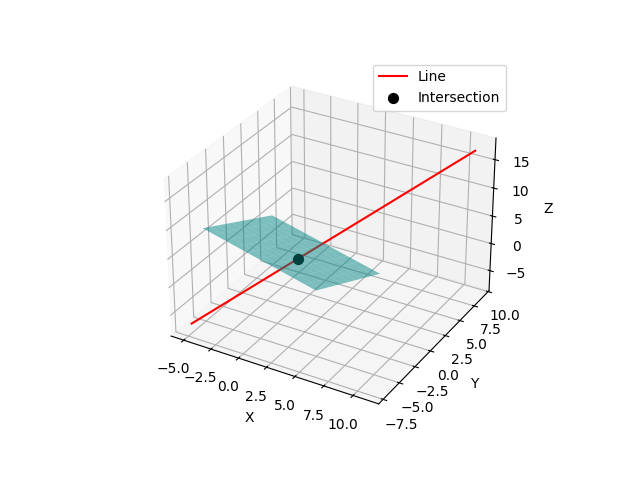
\includegraphics[width=0.65\columnwidth]{figs/1.png}
    \caption{}
\end{figure}

\end{document}

